\documentclass{article}

% Recommended ICML packages.
\usepackage{microtype}
\usepackage{graphicx}
\usepackage{subcaption}
\usepackage{booktabs}
\usepackage{hyperref}
\usepackage{amsmath}
\usepackage{amssymb}
\usepackage{mathtools}
\usepackage{placeins}
\usepackage{float}
\usepackage{xcolor}
\usepackage[capitalize,noabbrev]{cleveref}

% Keep draft pages dense. The paper prioritizes avoiding large blank regions;
% figures may float slightly past their source subsection when needed.
\setcounter{topnumber}{5}
\setcounter{bottomnumber}{4}
\setcounter{totalnumber}{10}
\setcounter{dbltopnumber}{4}
\renewcommand{\topfraction}{0.98}
\renewcommand{\bottomfraction}{0.90}
\renewcommand{\textfraction}{0.02}
\renewcommand{\floatpagefraction}{0.70}
\renewcommand{\dbltopfraction}{0.98}
\renewcommand{\dblfloatpagefraction}{0.70}

% Blind workshop submission. If accepted, switch to:
% \usepackage[accepted]{icml2026}
\usepackage{icml2026}

% Local notation. Keep custom macros minimal and do not use them in the title.
\newcommand{\zscore}{\ensuremath{z = (x-\mu)/\sigma}}
\newcommand{\primalz}{\ensuremath{d^{\mathrm{primal}}_{z}}}
\newcommand{\primalx}{\ensuremath{d^{\mathrm{primal}}_{x}}}
\newcommand{\logitdiff}{\ensuremath{\Delta_{\mathrm{logit}}}}
\newcommand{\redtodo}[1]{\textcolor{red}{\textbf{[TODO]} #1}}

\icmltitlerunning{The Geometry of Relativity}

\begin{document}

\twocolumn[
  \icmltitle{The Geometry of Relativity: Context-Normalized Encoding of Gradable Adjectives in LLMs}

  % The style file suppresses author information in the blind version.
  \begin{icmlauthorlist}
    \icmlauthor{Anonymous Authors}{anon}
  \end{icmlauthorlist}

  \icmlaffiliation{anon}{Anonymous Institution}
  \icmlcorrespondingauthor{Anonymous Authors}{anonymous@example.com}
  \icmlkeywords{mechanistic interpretability, representation geometry, language models, gradable adjectives}

  \vskip 0.3in
]

% Required by the ICML style, even for anonymous submissions.
\printAffiliationsAndNotice{}

% \noindent\textbf{Draft note.} This file is a structural scaffold, not submission prose.
% Every paragraph, claim, and citation must be rewritten and source-audited by a human before submission.
% Remove this note before uploading to OpenReview.

\begin{abstract}
Large language models make context-sensitive scalar judgments: the same value can be described differently depending on the comparison class described in the prompt.
We study whether this behavior reflects an internal representation of relative standings rather than raw magnitudes across a host of gradable adjectives such as \emph{tall}, \emph{rich}, and \emph{fast}. 
In this paper, we provide an overview of the subspaces that govern how Gemma 2 handles relativity in context, and show evidence through an intervention based approach that this relativity mechanism transcends any individual lexical adjective.
We do this through examining the internal representations of the variable expressed as itself and transformed into a normalized Z-score, and show the latter is more linearly decodable and correlated to adjective logit differences.
We then further provide evidence through showing that primal and dual based steering, as well as attention based ablations, generalize across Z-score transformations of concepts. We demonstrate this behavior in 5 model families and 8 separate feature categories. 
Overall, our results show that language models construct a context-relative scalar representation that is behaviorally dominant, internally accessible, and causally relevant, but not fully captured by a single universal direction. 
\end{abstract}

\section{Introduction}
\label{sec:introduction}

Gradable adjectives are context dependent.
A person who is $170$ cm tall can be described as tall in one comparison class and short in another.
This paper uses that everyday ambiguity as a controlled testbed for a mechanistic question: when a language model makes a scalar judgment from in-context examples, does it rely on the raw number, a learned world prior, or an internally constructed relative variable?

We formalize the target variable as a context-normalized standing,
\[
z=(x-\mu)/\sigma,
\]
where $x$ is the target value and $(\mu,\sigma)$ describe the comparison class that generated the prompt examples.
The experimental design deliberately samples $x$ and $z$ independently, then derives $\mu$, so that raw value and relative standing are not accidentally confounded.
This lets us ask whether the model's adjective logit difference follows ``$170$ cm'' or ``above the local norm.''

The main empirical picture is that Gemma 2 behaves as though a $z$-like variable is available.
Dense prompt grids show that adjective logits track $z$ much more strongly than raw $x$.
Cell-mean activation geometry is organized by the same variable.
Layerwise analyses suggest an encode/use separation: $z$ is linearly readable in early layers, while direct steering with \primalz{} has larger effects later.
Cross-concept transfer is positive but incomplete, and lexical decomposition shows why: part of the direction is shared across concepts, but same-concept steering also benefits from lexical and output-facing components.

The intended contribution is therefore not a claim of a pure universal relativity vector or a fully localized circuit.
Instead, we provide a claim ledger for a concrete relational computation: context examples induce a normalized scalar variable; that variable is visible in residual-stream geometry; it can be causally steered; and its cross-domain transfer is partially, but not completely, separable from lexical adjective structure.

\section{Setup and Experimental Design}
\label{sec:setup}

\subsection{Task and Variables}
\label{subsec:task-variables}

We study prompts that ask a model to complete a gradable adjective judgment after seeing a local comparison class.
For each prompt, we separate the raw value, the context, and the target's relative standing:
\begin{itemize}
  \setlength{\itemsep}{0pt}
  \setlength{\parskip}{0pt}
  \item \textbf{$x$:} raw target value, e.g. $170$ cm.
  \item \textbf{$\mu$:} context mean, e.g. the group average height.
  \item \textbf{$\sigma$:} context spread.
  \item \textbf{$z$:} context-normalized standing.
\end{itemize}
\[
z = \frac{x-\mu}{\sigma}.
\]
A model using only $x$ says ``170 cm is tall'' regardless of the group.
A model using $z$ says ``170 cm is tall in a short group, average in an average group, and short in a very tall group.''
The main behavioral measurement is the high-minus-low adjective logit difference:
\[
\logitdiff = \mathrm{logit}(\text{high adjective}) -
\mathrm{logit}(\text{low adjective}).
\]
For height, for example:
\[
\logitdiff=\mathrm{logit}(\text{tall})-\mathrm{logit}(\text{short}).
\]
Positive values mean the model leans toward the high adjective.

\begin{figure}[H]
  \centering
  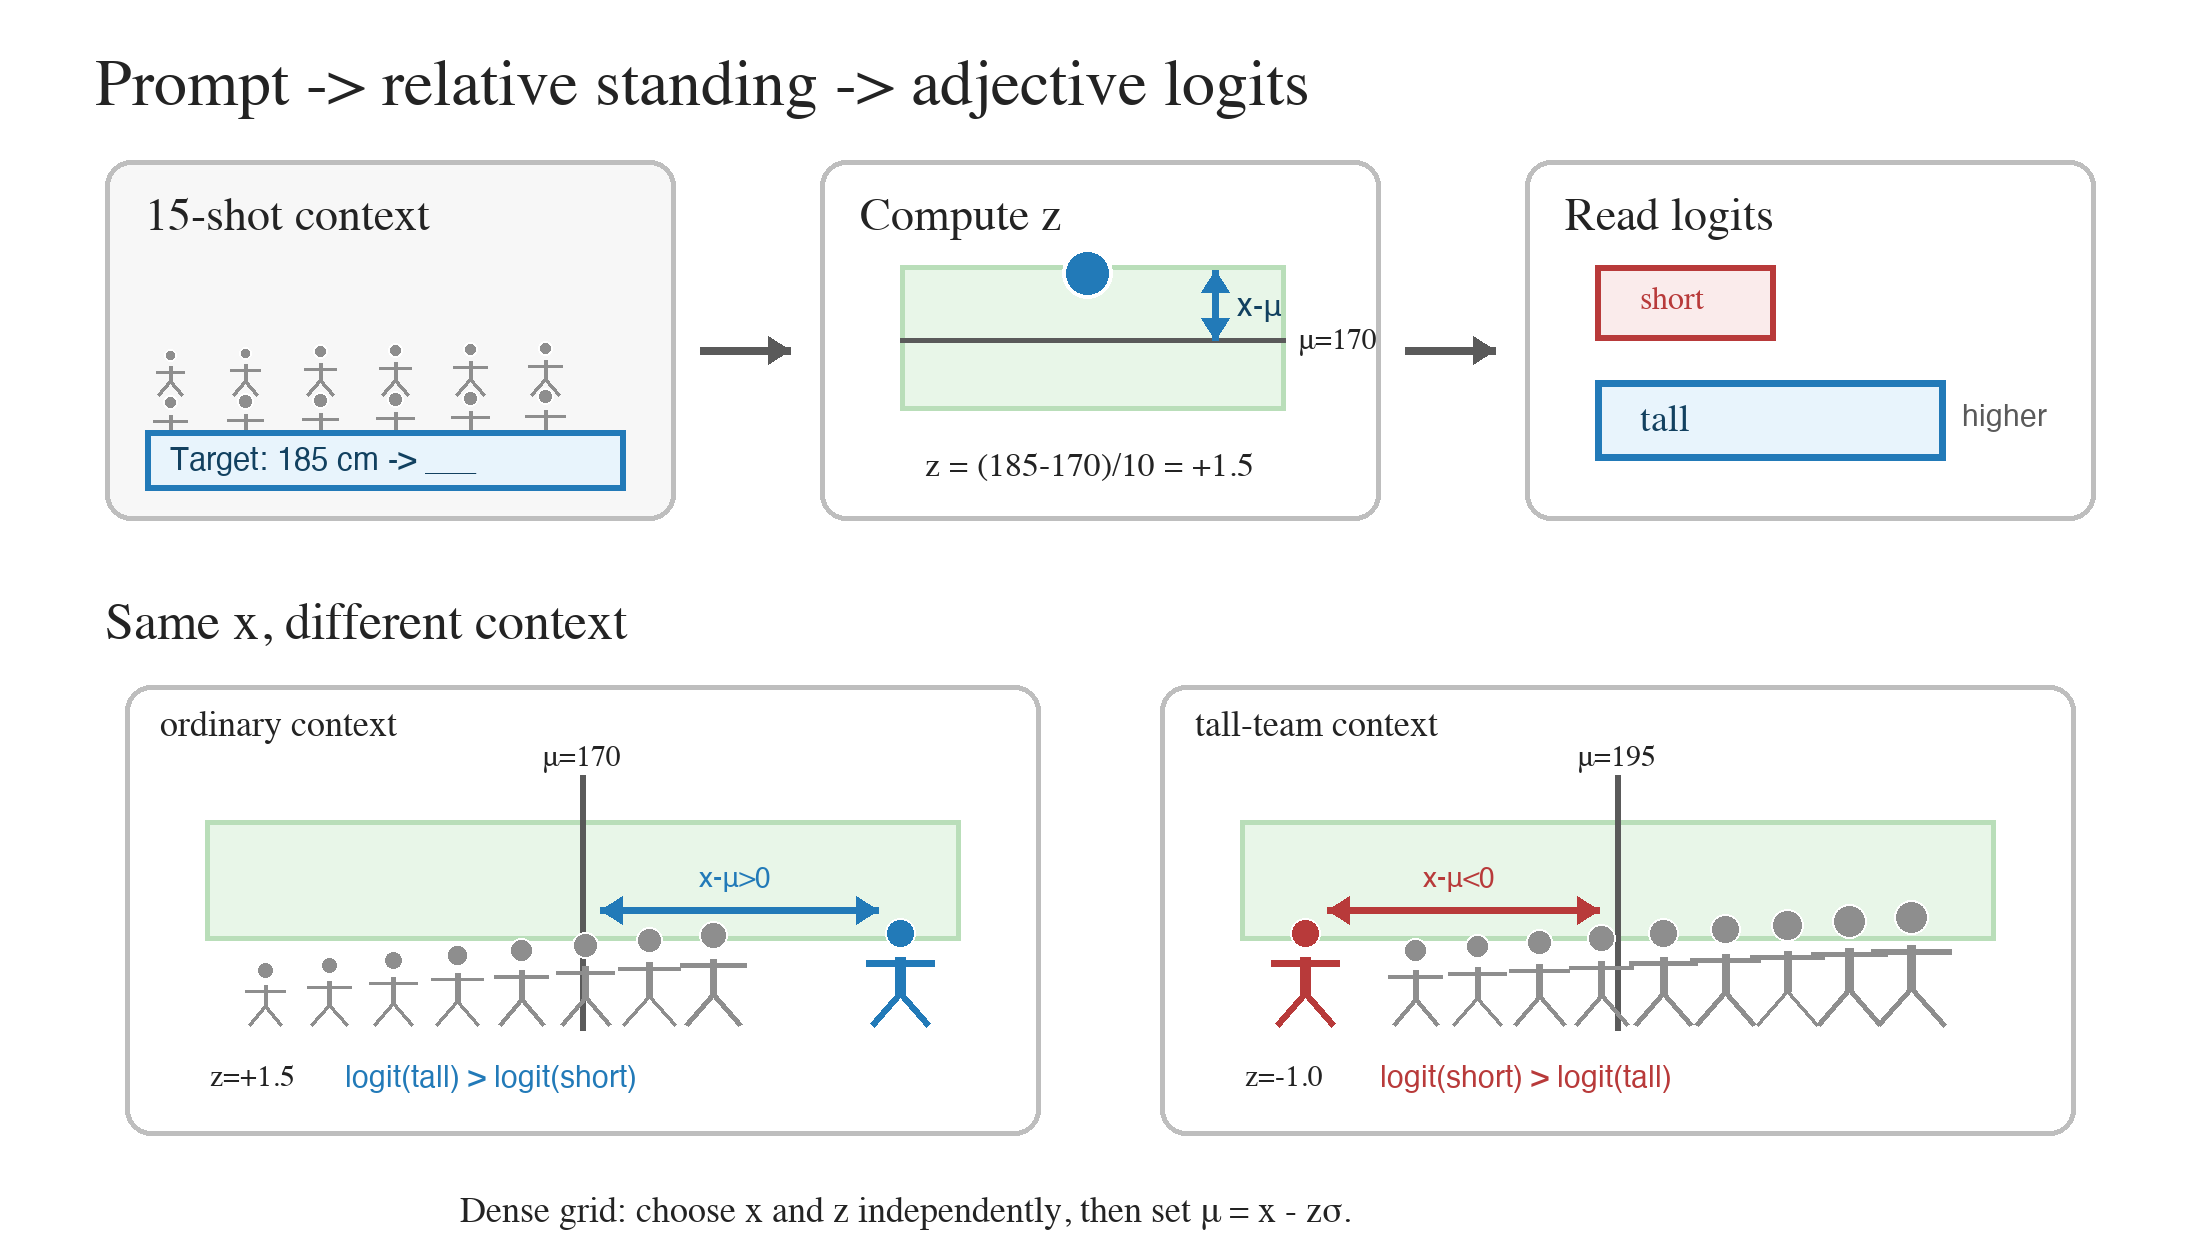
\includegraphics[width=\linewidth]{figures/fig1_prompt_schematic.png}
  \caption{\textbf{Prompt and measurement schematic.}
  Context examples define a local comparison class.
  We compute the target's normalized standing $z=(x-\mu)/\sigma$ and measure whether the model assigns higher logit to the high adjective or the low adjective.
  The same raw value can support opposite completions under different context means, motivating a dense grid that separates $x$ from $z$.
  % Source asset: paper/icml2026_draft/figures/candidates_png/candidate_5_combined_pipeline_relcontrast.png.
  }
  \label{fig:setup-pipeline}
\end{figure}

\begin{table}[H]
  \centering
  \scriptsize
  \setlength{\tabcolsep}{3pt}
  \begin{tabular}{lllll}
    \toprule
    Concept & Unit & Low/High & $\sigma$ & $x$ range \\
    \midrule
    Height & cm & short/tall & 10 & 147--183 \\
    Age & yr & young/old & 5 & 16--64 \\
    Weight & kg & light/heavy & 8 & 45--105 \\
    Size & cm diameter & small/big & 6 & 0.5--65.5 \\
    Speed & km/h & slow/fast & 15 & 7--163 \\
    Income & $\log(\mathrm{USD/yr})$ & poor/rich & $\log 2$ & \$14k--\$900k \\
    Experience & years & novice/expert & 4 & 0.5--27.4 \\
    BMI & kg/m$^2$ & thin/obese & 3 & 14.9--40.1 \\
    \bottomrule
  \end{tabular}
  \caption{\textbf{Adjective-pair prompt domains.}
  The dense prompt grid samples target values $x$ over the listed ranges, in the listed units, and uses the shown context spread $\sigma$.
  Income is used as the measured proxy for wealth; its normalization is log-space, so $\sigma=\log 2$ means one unit of normalized spread corresponds to doubling or halving annual income.}
  \label{tab:domains}
\end{table}
\FloatBarrier

\subsection{Prompt Regimes}

% TODO(human): Decide final wording after the shot-sweep results are integrated.
The paper compares prompt regimes that vary how much comparison-class evidence is available:
zero-shot prompts with only the target value, few-shot prompts with a small number of context examples, and dense 15-shot prompts.
The shot-sweep experiments make this distinction central: raw-value behavior is strongest with no context, while context-relative behavior strengthens once examples are supplied.

\subsection{Dense Grid Construction}
\label{subsec:dense-grid}

The dense grid samples $x$ and $z$ independently, then derives the context mean:
\[
\mu = x - z\sigma.
\]
This design prevents raw value and relative standing from being accidentally confounded.
After choosing $(x,z)$ and deriving $\mu$, an $N$-shot prompt draws context examples from the population distribution
\[
c_1,\ldots,c_N \sim \mathcal{N}(\mu,\sigma^2),
\]
then renders those samples in the same unit as the target.
Thus $z$ is the target's standing relative to the population parameters that generated the comparison class, while different context seeds instantiate different sampled groups.
The current dense-grid setting uses 20 target values, 20 target $z$ values, and 10 context seeds per adjective pair, with the main dense prompts using 15 context examples.
% TODO(source): Verify final sample counts after dropped implausible cells are accounted for.
For income, the analogous definition is log-space:
\[
z = \frac{\log x - \log \mu}{\log 2}.
\]

\subsection{Models, Concepts, and Measurements}
\label{subsec:models-concepts-measurements}

The current evidence focuses on Gemma 2 2B and Gemma 2 9B.
The main concept set contains eight adjective pairs: height, age, weight, size, speed, income/wealth, experience, and BMI/obesity.
Measurements include logit differences, residual-stream activations, PCA and linear-probe readouts, steering interventions, lexical/residual decompositions, SAE feature audits, and attention/ablation analyses.
% TODO(source): Move exact model IDs, layer counts, prompt templates, activation sites, steering scales, and seeds to the appendix.
% TODO(human): Decide which additional domains/objective controls enter the final main text.

For concept pair $p$ and layer $L$, we use \primalz{} for the high-margin mean-difference direction that contrasts above-norm and below-norm prompts:
\[
d^{\mathrm{primal}}_{z,p,L}
= \mathbb{E}[h_L \mid p, z>1]
- \mathbb{E}[h_L \mid p, z<-1].
\]
The raw-value control \primalx{} is defined analogously by contrasting high-$x$ and low-$x$ prompts.
These are descriptive residual-stream directions used for steering and transfer; they are not supervised probe weights.

\subsection{Evidence Types}
\label{subsec:evidence-types}

The results distinguish behavioral evidence, linear availability, geometry, causal intervention, and decomposition.
Behavioral correlations show what the model outputs; probes show what is linearly available; PCA describes geometry; steering and ablations test causal relevance; lexical and SAE analyses test alternative explanations.
% TODO(human): Keep this paragraph short; the main results should instantiate each evidence type rather than over-explaining it here.

\section{Results}
\label{sec:evidence}

\subsection{Context Examples Shift Judgments Toward $z$}
\label{subsec:behavioral-grids}

We first ask whether the model's adjective preference follows raw value $x$ or context-normalized standing $z$.
Across the dense prompt grid, cell-mean logit differences are strongly correlated with $z$ for every tested adjective pair.
This is the behavioral anchor for the paper: once a comparison class is present, the target value alone is not sufficient to explain the adjective readout.

\begin{table}[!tbp]
  \centering
  \footnotesize
  \setlength{\tabcolsep}{4pt}
  \begin{tabular}{lrr}
    \toprule
    Concept & corr$(\logitdiff,z)$ & corr$(\logitdiff,x)$ \\
    \midrule
    Height & \textbf{0.976} & 0.107 \\
    Age & \textbf{0.940} & -0.002 \\
    Weight & \textbf{0.967} & 0.114 \\
    Size & \textbf{0.928} & 0.366 \\
    Speed & \textbf{0.930} & 0.412 \\
    Income & \textbf{0.964} & 0.260 \\
    Experience & \textbf{0.951} & 0.356 \\
    BMI & \textbf{0.954} & 0.216 \\
    \bottomrule
  \end{tabular}
  \caption{\textbf{Adjective behavior tracks relative standing.}
  After averaging over context seeds within each $(x,z)$ cell, high-minus-low adjective logit differences correlate more strongly with $z$ than with raw $x$.
  % Source: internal/kshot/phase/FINDINGS.md Phase 0 reproduction table.
  }
  \label{tab:behavioral-z-corr}
\end{table}

The height grid in \cref{fig:dense-height-heatmap} gives the simplest visual readout of the same result.
When raw height and $z$ are sampled independently, the tall-minus-short logit difference varies primarily along the context-normalized axis.

\begin{figure}[!tbp]
  \centering
  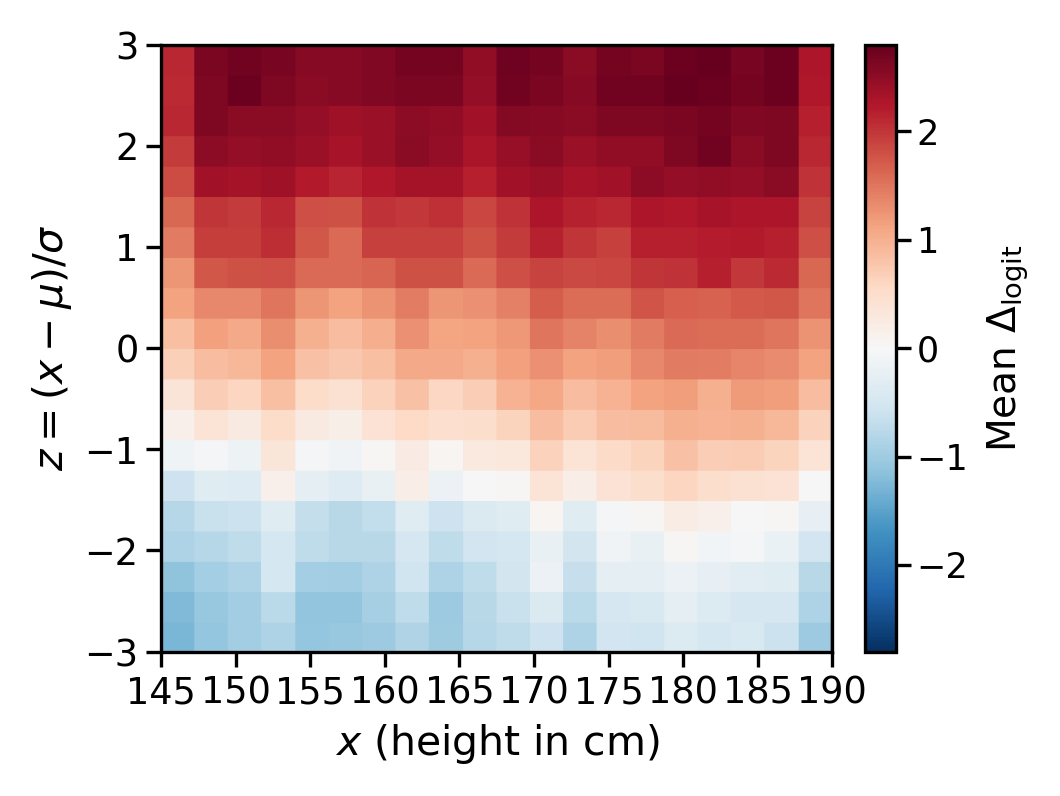
\includegraphics[width=\linewidth]{figures/fig_results_dense_height_heatmap_clean.png}
  \caption{\textbf{Dense height grid.}
  In a controlled grid where raw height $x$ and relative standing $z$ are separated, the model's high-minus-low adjective logit difference changes mostly with $z$.
  % Source artifact: figures/v10/behavioral_logit_diff_xz.png, cleaned for paper display.
  }
  \label{fig:dense-height-heatmap}
\end{figure}

\Cref{fig:pca-montage} shows the same organization in activations.
PCA on cell-mean residual-stream activations shows ordered arcs across adjective domains: nearby points have similar context-normalized standing even when their raw units and adjectives differ.
This visualization is descriptive rather than causal, but it motivates the probe and steering tests below.

\begin{figure}[!tbp]
  \centering
  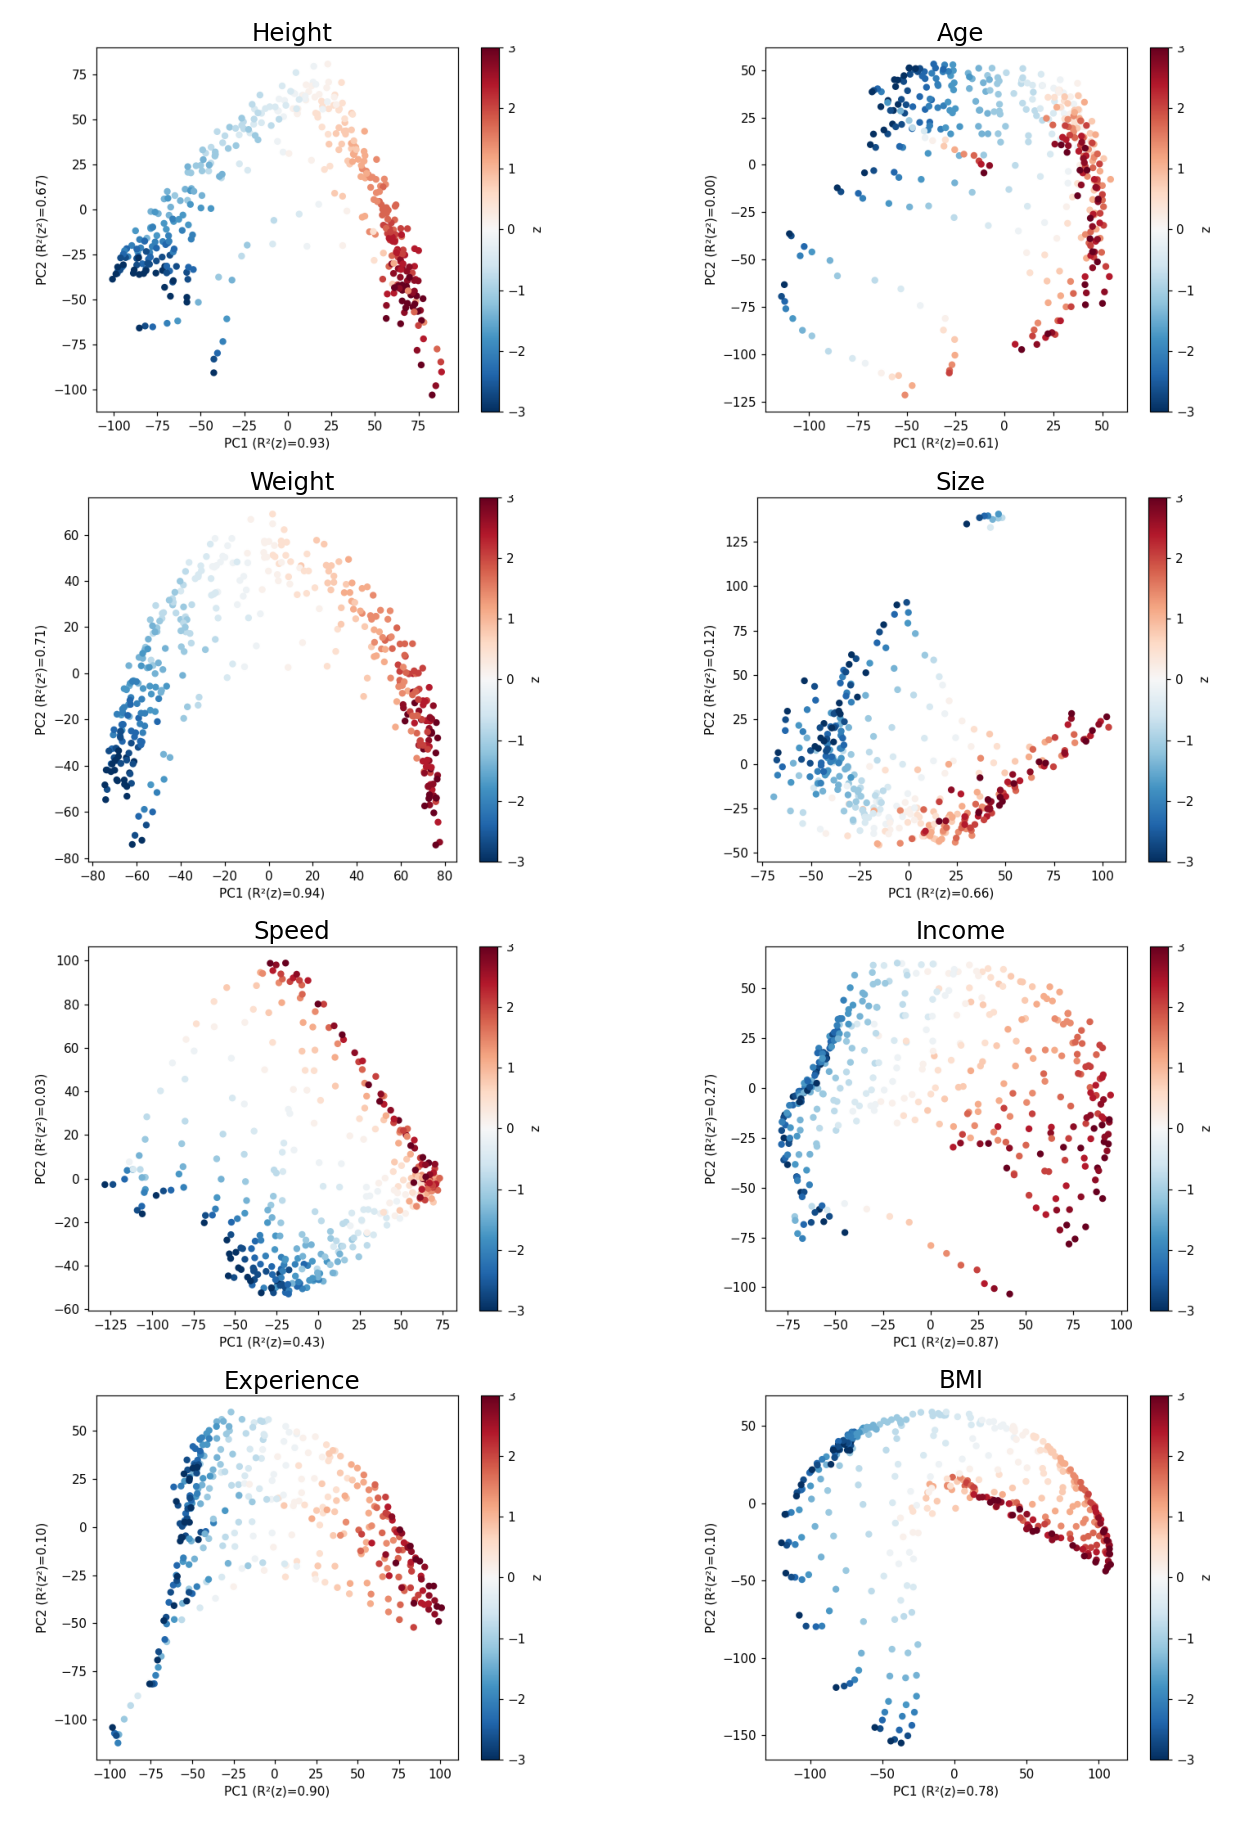
\includegraphics[width=\linewidth]{figures/fig_results_pca_all_pairs_clean.png}
  \caption{\textbf{Cell-mean activation geometry.}
  Late-layer PCA views of all eight dense prompt domains show ordered $z$ structure across adjective domains.
  The plot is geometry evidence, not by itself a mechanism claim.
  % Source artifacts: figures/v11/pca/*_gemma2-9b_2d_L33.png, cleaned and relabeled for paper display.
  }
  \label{fig:pca-montage}
\end{figure}

\Cref{fig:kshot-ld-evolution} shows that prompt regime matters.
With no comparison examples, raw-value priors dominate; as context examples are added, the same judgment becomes organized by effective relative standing.

\begin{figure}[!tbp]
  \centering
  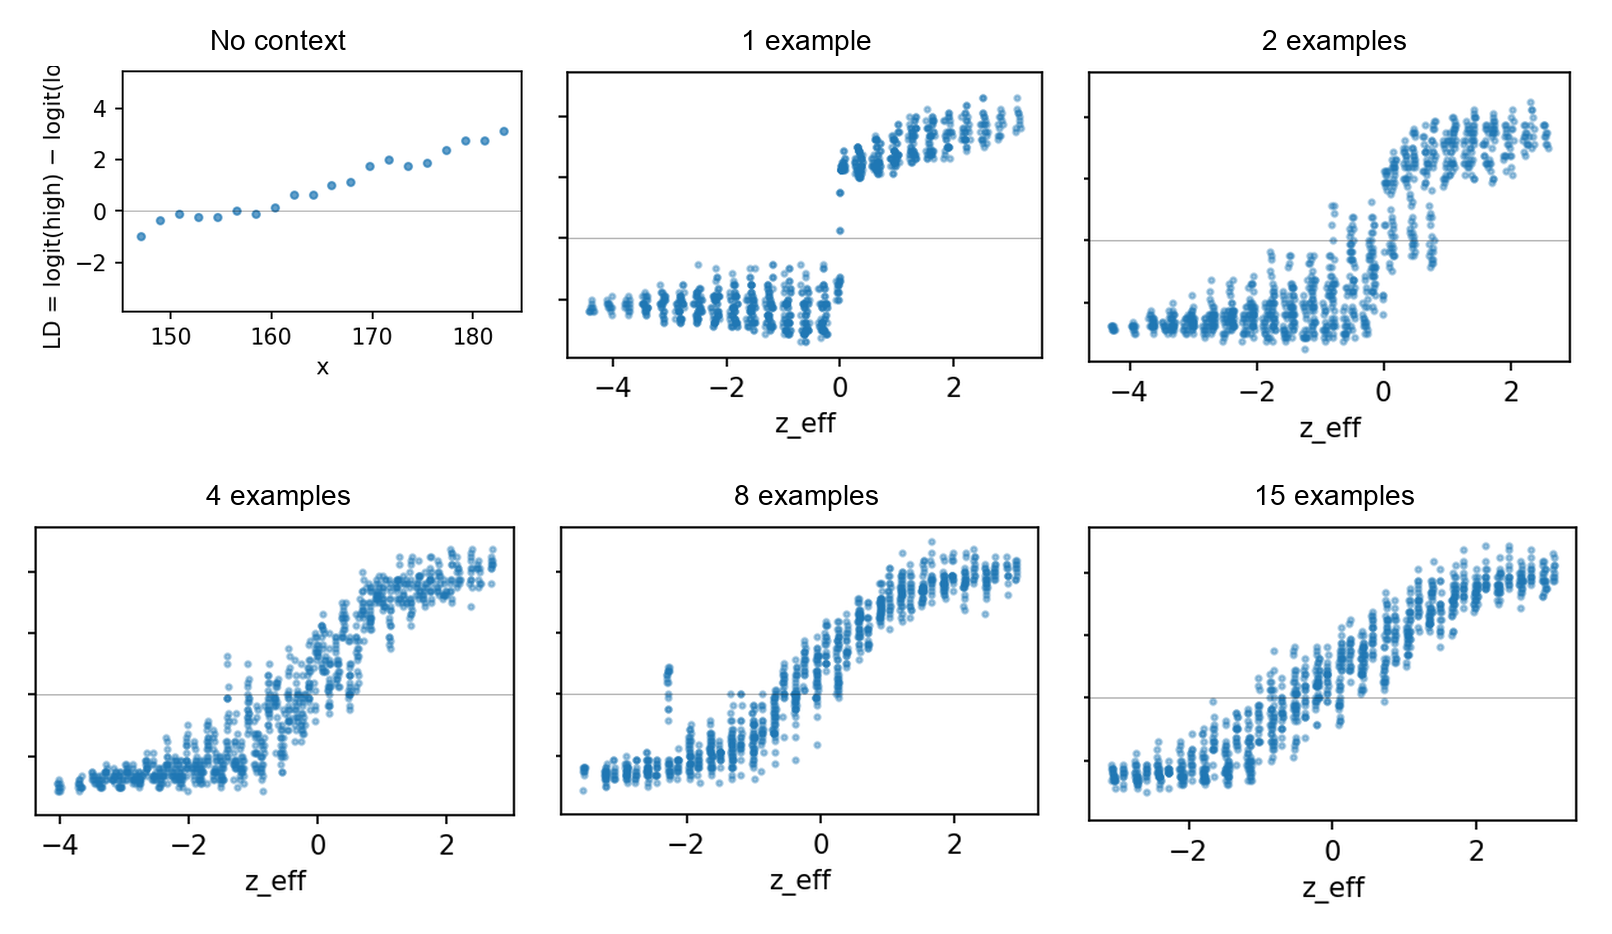
\includegraphics[width=\linewidth]{figures/fig_results_kshot_ld_evolution_2x3.png}
  \caption{\textbf{Logit-difference evolution with context length.}
  With no context examples, the height judgment is organized by raw height $x$.
  After context examples are added, the same logit difference becomes organized by effective relative standing and changes from a sharp comparator-like pattern toward a smoother graded response.
  % Source artifact: internal/kshot/phase/figures/p2a_ld_vs_z_height_gemma2-9b.png, reformatted as a one-column 2-by-3 plot.
  }
  \label{fig:kshot-ld-evolution}
\end{figure}

% TODO(control): Add OOD/extreme-value results here if the affine-shift experiments survive review.

\subsection{Internals: $z$ Is Encoded Early and Used Later}
\label{subsec:layer-evolution}

\Cref{fig:layer-encode-use} summarizes the current internal evidence for an encode/use separation.
Linear readouts recover $z$ in early layers, while direct residual-stream steering with the \primalz{} direction is strongest in later layers.
This should be phrased as a layerwise readout/intervention pattern, not as a fully localized circuit.

\begin{figure}[!tbp]
  \centering
  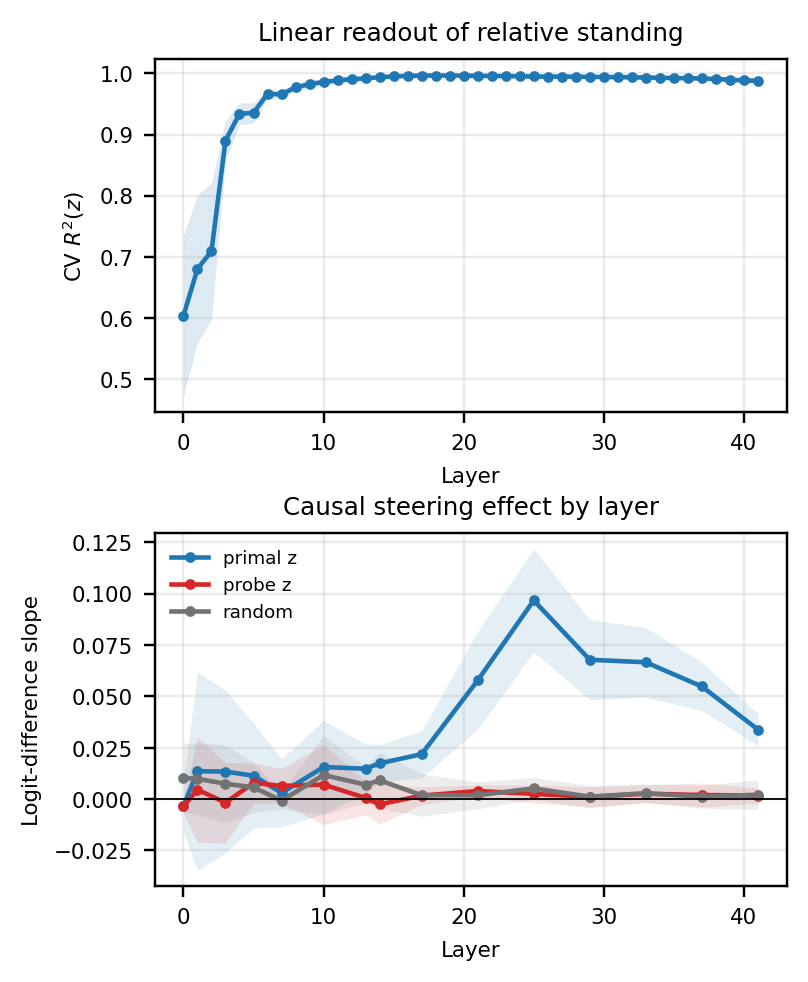
\includegraphics[width=\linewidth]{figures/fig_results_layer_sweep_summary_clean.png}
  \caption{\textbf{The context-normalized variable is available early but most causally potent later.}
  Linear availability of $z$ rises quickly in early layers, while direct \primalz{} steering has its largest effect later.
  This separates decodability from use: a variable can be linearly readable before it is the most effective causal steering direction.
  % Source artifact: figures/v12/layer_sweep_9b_combined.png, cleaned for paper display.
  }
  \label{fig:layer-encode-use}
\end{figure}

The next mechanism question is how the context examples are turned into that variable.
The working story is that the model behaves partly like a Bayesian data scientist: it reads the context values, forms a comparison statistic, and applies the resulting standing to the target.
We find it useful to understand how a model is operating to abstract two scales of "relativistic" and "objective" behavior, and visualize this as a 2d plane as per \Cref{fig:relative-objective-phase}.
Quantitativiely, we can measure both relativity and objectivity by looking at the partial correlations to z and x respectively. That is to say, a vertical axis measures relative use, $\mathrm{corr}(\mathrm{LD},z\mid x)$, while a horizontal axis measures objective/raw-value use, $\mathrm{corr}(\mathrm{LD},x\mid z)$.
With no context, the model operates in a purely objective state, with heights above 160cm already preferring tall compared to short. 
As more context examples are supplied, baseline behavior moves toward the relativistic region, becoming a direct comparison operation. As more context is saturated, the model reintegrates it's objective capabilities with its relativistic context.

\begin{figure}[!tbp]
  \centering
  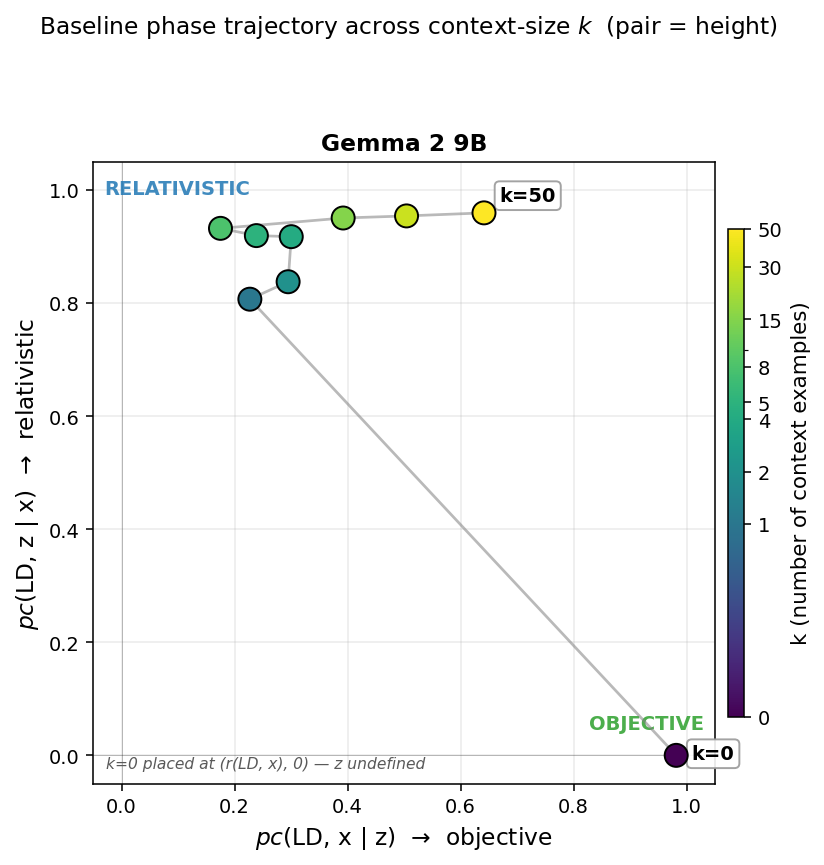
\includegraphics[width=\linewidth]{figures/p2d_phase_k_sweep_9b.png}
  \caption{\textbf{Relative/objective phase plane for shot-sweep.}
  We can see how Gemma2 9B model behavior changes as we introduce more relativistic context. It only takes one example for the model to become extremely relativistic, with more context generally leading to the model reintegrating its objective view as well.
  % Source artifacts: internal/kshot/phase/results/p2d_l0all_per_k_gemma2-9b_height.json, p2d_partial_l0_gemma2-9b_height_k1.json, and p2e_residual_interventions_gemma2-9b_height_k15.json, replotted for paper display.
  }
  \label{fig:relative-objective-phase}
\end{figure}

\subsection{A Shared $z$ Direction Partly Transfers Across Concepts}
\label{subsec:shared-direction}

We next ask whether each adjective pair has its own private direction, or whether a shared $z$-like relativity component transfers across concepts.
\Cref{fig:shared-direction-steering} shows that a Procrustes-aligned shared direction steers most concepts in the expected direction.
In the 9B model, the mean pairwise cosine among pair-specific \primalz{} directions is $0.52$, the shared direction has cosine $0.64$--$0.90$ with individual pair directions, and shared-direction steering reaches at least half of within-pair steering for $7/8$ pairs.

\begin{figure}[!tbp]
  \centering
  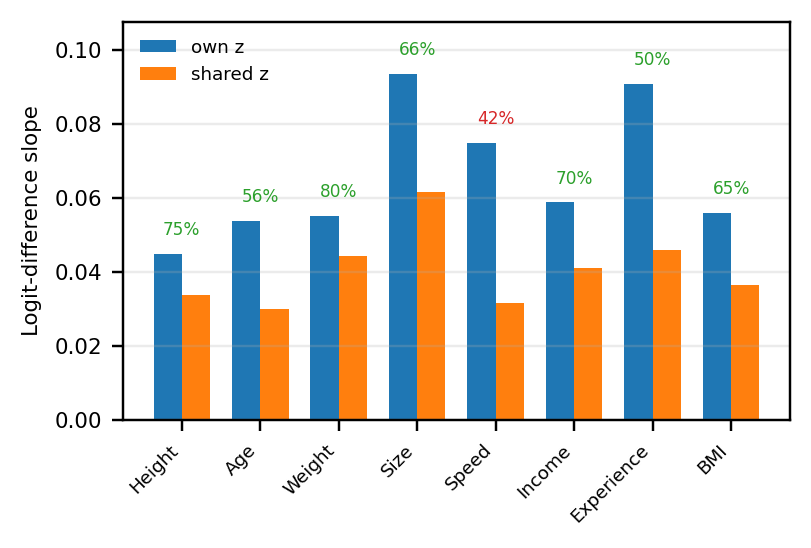
\includegraphics[width=\linewidth]{figures/fig_results_shared_direction_steering_clean.png}
  \caption{\textbf{A shared direction preserves much of within-concept steering.}
  For each concept, the plot compares steering with the concept's own \primalz{} direction against steering with a single Procrustes-aligned shared direction.
  Ratios above $0.5$ mean the shared direction recovers at least half of the same-concept effect.
  % Source artifact: results/v11_5/gemma2-9b/shared_z_analysis.json, replotted for paper display.
  }
  \label{fig:shared-direction-steering}
\end{figure}

Second, \cref{fig:z-vs-x-transfer} shows that steering with a source concept's \primalz{} direction often shifts the target concept in the expected high-minus-low direction.
The diagonal entries are strongest, as expected, but off-diagonal transfer is consistently positive in the current dense-grid runs.
The raw-value control makes the comparison sharper: when we repeat the same 8-by-8 transfer experiment using raw-$x$ directions, transfer is much weaker.

\begin{figure}[!tbp]
  \centering
  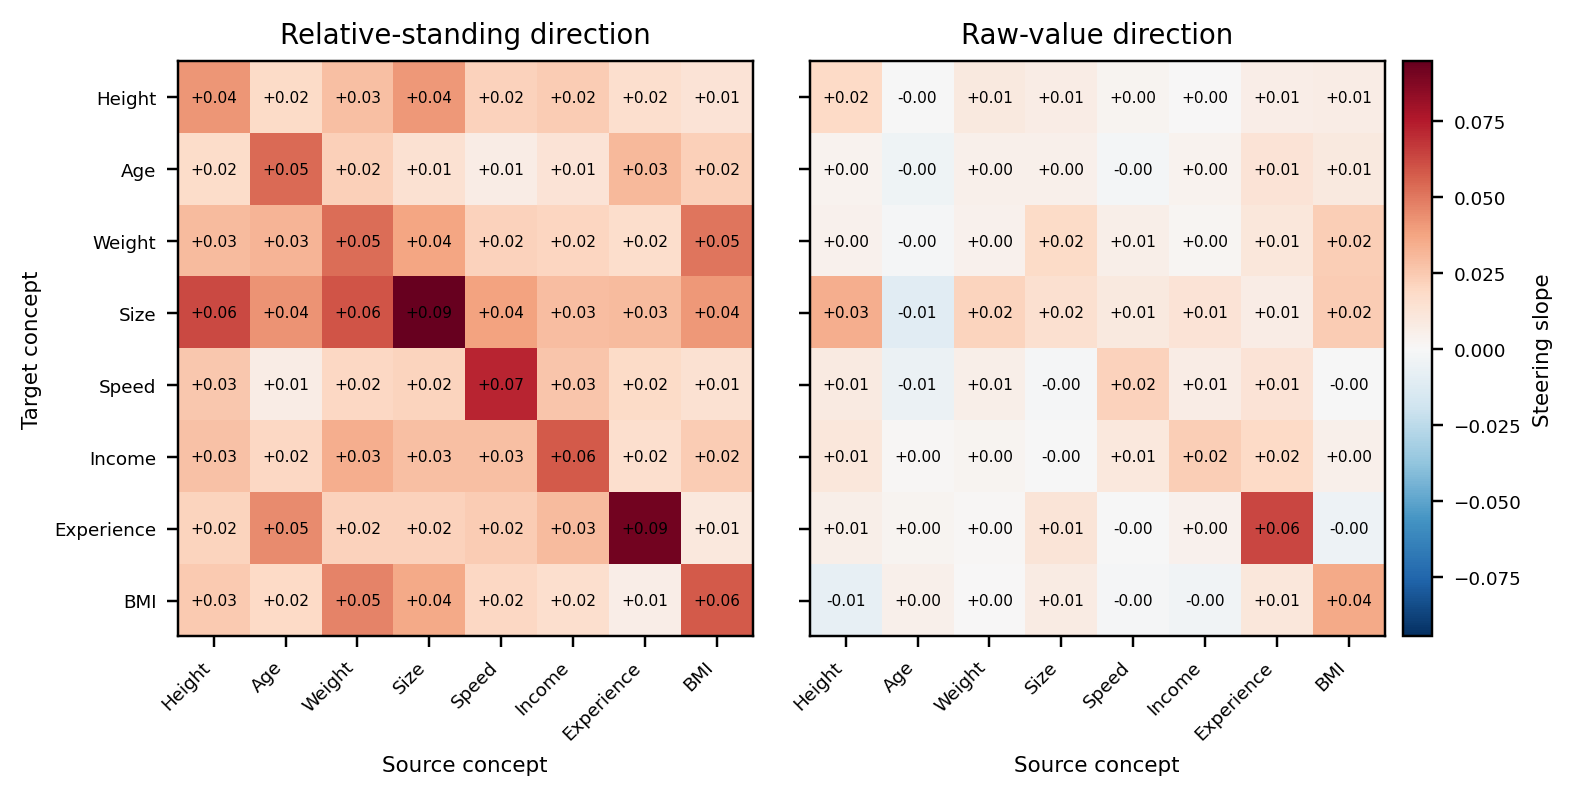
\includegraphics[width=\linewidth]{figures/fig_results_z_vs_x_transfer_clean.png}
  \caption{\textbf{$z$ directions transfer more broadly than raw-value directions.}
  Rows are target concepts and columns are source concepts.
  The left heatmap steers with source-concept \primalz{} directions; the right heatmap uses source-concept raw-$x$ directions.
  Mean off-diagonal transfer is $+0.026$ for $z$ directions versus $+0.006$ for raw-value directions.
  % Source artifact: raw-value transfer control JSON, replotted for paper display.
  }
  \label{fig:z-vs-x-transfer}
\end{figure}

The safe interpretation is partial transfer, not a pure universal code.
For the 9B model, the mean diagonal steering slope is about $0.066$, while the mean off-diagonal slope is about $0.026$.
That means cross-concept steering recovers roughly $40\%$ of the same-concept effect on average.
The remaining gap is important: concept-specific lexical and output-facing components still matter.

To test this, \cref{fig:lexical-residual,fig:lexical-residual-matrices} decomposes each pair's context-derived direction into a tested lexical subspace and an orthogonal residual:
\[
p_z = p_{z,\mathrm{lex}} + p_{z,\mathrm{resid}}.
\]
The lexical subspace is built from adjective-token, adjective-in-sentence, sentence-final, synonym, and domain-token directions.
Literal adjective-token directions align only weakly with \primalz{}:
mean cosine is $0.104$ for word-token directions, $0.102$ for sentence-token directions, and $0.260$ for sentence-final directions.
Only about $8\%$ of \primalz{} norm-squared lies in the tested lexical subspace, but the normalized lexical projection is high-gain for same-concept steering.

\begin{figure}[!tbp]
  \centering
  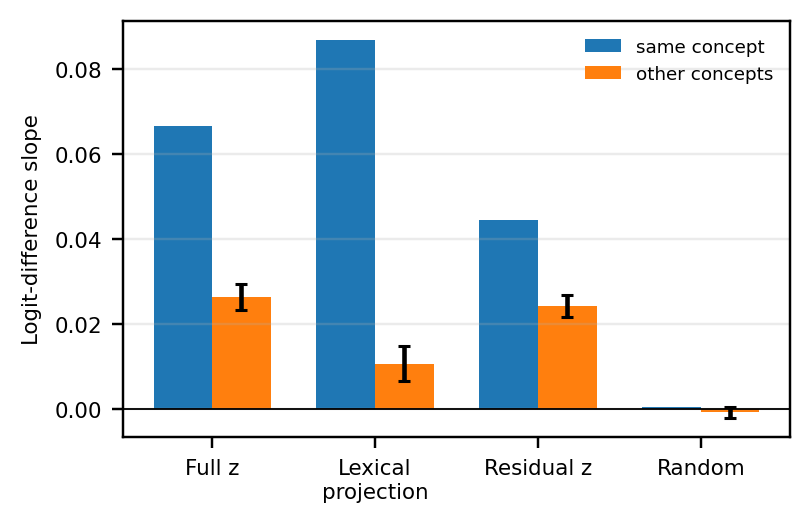
\includegraphics[width=\linewidth]{figures/fig_results_lexical_transfer_summary_clean.png}
  \caption{\textbf{Shared transfer is not purely lexical.}
  Projecting onto a lexical adjective subspace gives strong same-concept steering but weak transfer to other concepts.
  Removing that lexical projection leaves a residual direction with weaker same-concept steering but relatively stronger cross-concept transfer.
  % Source artifact: results/v12_2/residual_vs_lexical_transfer_summary.json, replotted for paper display.
  }
  \label{fig:lexical-residual}
\end{figure}

\begin{figure}[!tbp]
  \centering
  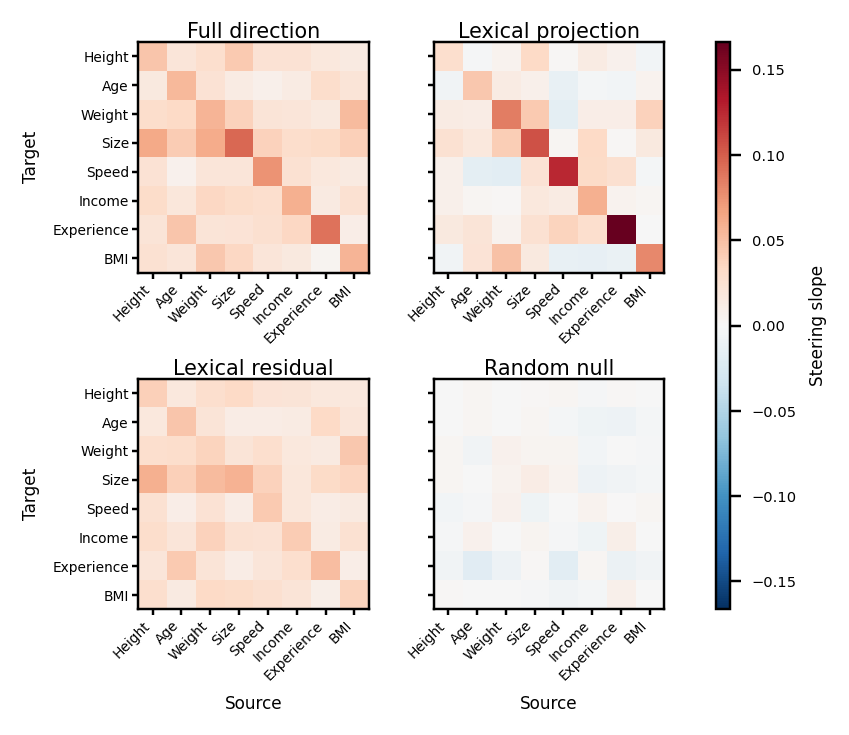
\includegraphics[width=\linewidth]{figures/fig_results_residual_vs_lexical_transfer_matrices_clean.png}
  \caption{\textbf{Residual and lexical cross-pair transfer matrices.}
  The full \primalz{} direction transfers broadly, the lexical projection is strongest on same-concept cells, and the lexical residual preserves more off-diagonal transfer.
  The random null remains near zero.
  % Source artifact: results/v12_2/residual_vs_lexical_transfer.json, replotted for paper display.
  }
  \label{fig:lexical-residual-matrices}
\end{figure}

The residual transfers better off-diagonal than the lexical projection and recovers most of full \primalz{} transfer.
However, residual transfer still correlates with target lexical-subspace overlap ($r\approx 0.79$), so this is evidence for a residual shared component, not proof of a clean non-lexical shared code.
% TODO(experiment): Add semantically distant or objective control concepts if they survive the design review.

\subsection{Attention Based Interventions}
\label{subsec:attention}

Alongside conventional intervention methods such as primal and dual vector steering, we also demonstrate causality in attention based interventions in Gemma 2 2B. We experiment with choosing heads based on direct-logit-attribution (DLA) (Elhage et al., 2021. A Mathematical Framework for Transformer Circuits) scoring as well as cosine-similarity scoring to relativity as a direction expressed in SAE space. We furthermore experiment with ablating via zeroing heads, queries, or resampling heads. In particular, we are able to show that we are able to resample a small number of heads (e.g. 5 out of a total 208) to effectively destroy the relativity signal readout to logits whilst achieving minimal KL divergence on normal natural language prompts and other features. The same heads are responsible across all relativity concepts. 

We rank heads by direct logit attribution (DLA): for each head we project its last-token output through its $W_O$ slice into the unembedding difference $W_U[\text{tall}]-W_U[\text{short}]$ to obtain a per-prompt scalar contribution to the high--low logit split, and score the head by $\sigma_{\mathrm{DLA}} \cdot |\rho(\mathrm{DLA}, z)|$ --- the per-prompt standard deviation of that contribution times its correlation with the relativistic variable $z$. We restrict to heads with positive $\rho$, so that the ranking surfaces heads that move the readout in the same direction as $z$ rather than against it. As an independent ranking we decompose pre-$o_{\mathrm{proj}}$ head activations at all layers with the public Gemma Scope sparse autoencoders (SAEs), compute the cosine alignment between each candidate head's activation shift under zero-ablation and the dual-steered activation difference at the layer where the ablation is applied, and multiply by per-head std to obtain a comparable alignment-times-swap-distance score. The two rankings recover the same primary heads --- L16H4 as hub, L17H7 and L14H2 as cooperating partners --- but DLA is logit-grounded, computationally simpler and generally more effective. We therefore use DLA as the main ablation criteria.

The choice of ablation mechanism is load-bearing. Zero-ablation of any single L1 head --- including the head per-head correlation flags as the primary $z$-tracker --- produces $|\Delta r(\mathrm{LD}, z)| \le 0.001$ on Gemma 2 2B; whole-head zeroing, single SAE-feature subtraction, and Q-zeroing on isolated cells are all similarly null. We attribute this to redundancy: by mid-network the residual stream carries near-perfect linear information about $z$ at every head (cross-validated $R^2(z \mid \mathrm{head}) \ge 0.97$ for L8 and beyond), so zeroing any one contributor lets the others compensate. Resample (interchange) ablation --- replacing the head's last-token output with the same head's output drawn from a randomly chosen other prompt in the dataset --- instead preserves the head's contribution magnitude while corrupting the prompt-specific information it routes, and the corrupted output then propagates downstream to bias the readout toward the donor prompt. On the same cells, resample is consistently $15$--$25\times$ more damaging than zero. Throughout this section ``ablation'' therefore means interchange resample.

\begin{figure}[!tbp]
  \centering
  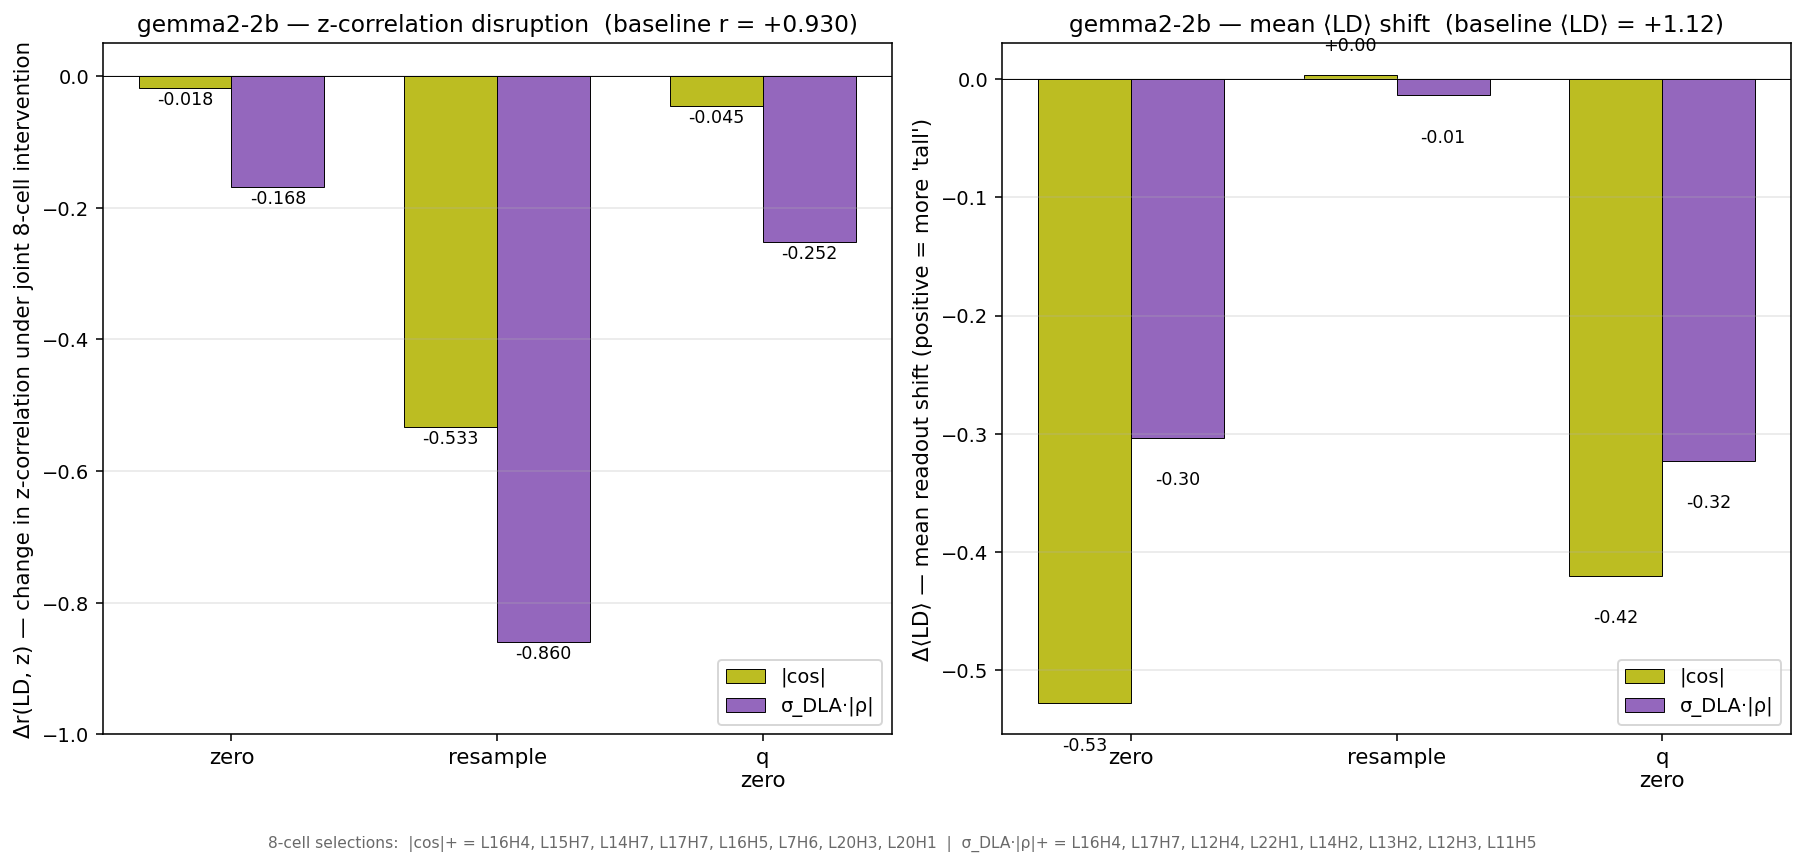
\includegraphics[width=\linewidth]{figures/p2o_attention_modes_comparison_gemma2-2b.png}
  \caption{\textbf{Intervention mode comparison on Gemma 2 2B (height, joint $8$-cell intervention).}
  Left: change in $r(\mathrm{LD},z)$ under three modes --- zero-ablation, interchange (resample), and query-zero --- for $8$-head selections by $|\mathrm{cos}|$ and $\sigma_{\mathrm{DLA}}\cdot|\rho|$ methods.
  Right: mean readout shift $\Delta\langle\mathrm{LD}\rangle$ (positive $=$ more ``tall'').
  Zero-ablation barely moves $z$-correlation but pushes the mean readout strongly toward a neutral readout; resample drains $z$-correlation while leaving the mean readout essentially unchanged.
  Resample is therefore the intervention used throughout this section: it isolates relativity.
  % Source artifact: relativity_ablation/figures/p2o_attention_modes_comparison_gemma2-2b.png.
  }
  \label{fig:intervention-modes}
\end{figure}

Greedy top-$N$ interchange ablation under $\sigma_{\mathrm{DLA}} \cdot |\rho|$ ranking drives $r(\mathrm{LD}, z)$ from the baseline $+0.93$ through zero into a slightly inverted $-0.12$ by $N{=}10$ on Gemma 2 2B (height, $k{=}15$). The cells entering the ablation set in $\sigma_{\mathrm{DLA}}$-ranked order also have monotonically decreasing cosine alignment to the SAE-space relativity direction (\cref{fig:circuit-trio}, right axis), providing intuition as to its effectiveness. The first eight cells account for roughly 84\% of the eventual $\Delta r$, and $\Delta r$ saturates entirely by $N{\approx}10$; beyond $N{=}10$, additional ablations do not further damage the relativity readout. The relativity circuit has a finite extent rather than a long tail.


\begin{figure}[!tbp]
  \centering
  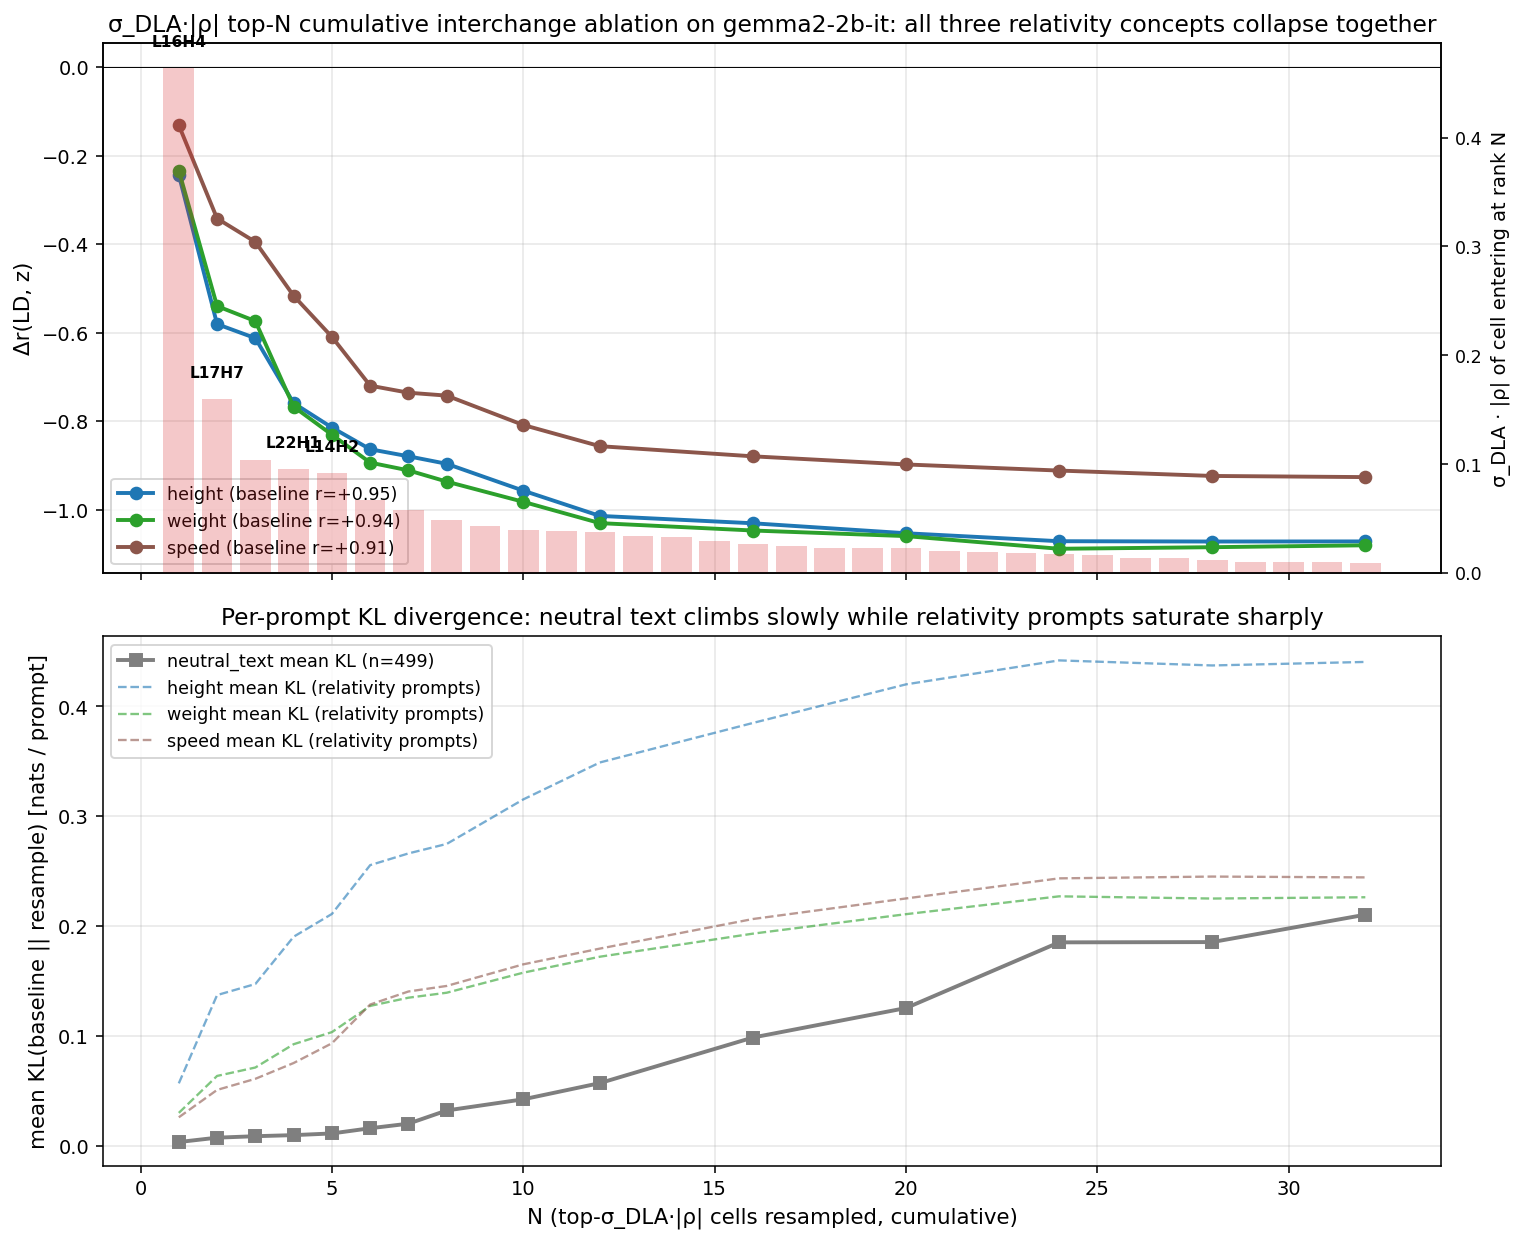
\includegraphics[width=\linewidth]{figures/p2u_n_sweep_xfeat_gemma2-2b-it.png}
  \caption{\textbf{DLA-ranked greedy ablation drives the model's $d_z$ alignment to zero on Gemma 2 2B.}
  Top: $\Delta r(\mathrm{LD},z)$ (left axis) over top-$N$ greedy resampling under $\sigma_{\mathrm{DLA}}\cdot\rho$ ranking, with the cos$\cdot\sigma$ of each newly added cell on the right axis.
  $\Delta r$ falls monotonically from a strongly positive baseline through zero into a slightly inverted readout, and the incoming cells' cos$\cdot\sigma$ values fall in tandem --- a visual readout that cosine alignment to $d_z$ is being progressively removed.
  Bottom: mean KL divergence between baseline and ablated next-token distributions, monotonically increasing.
  % Source artifact: relativity_ablation/figures/p2u_n_sweep_xfeat_gemma2-2b-it.png.
  }
  \label{fig:circuit-trio}
\end{figure}

The top 3 trio identified from the height grid transfers without re-derivation to the other relativity concepts: the joint resample of L16H4, L17H7 and L14H2 drops $r(\mathrm{LD}, z)$ by $0.57$ on height, $0.68$ on weight, and $0.47$ on speed --- $61$--$73\%$ of the baseline correlation in each case --- confirming that the circuit is relativity-general rather than tied to any one surface adjective. To test whether the trio simply damages the model's general competence, we ran the same intervention on three control tasks --- arithmetic comparison (``Is $X$ greater than $Y$?''), factual truth (Marks \& Tegmark cities, framed as ``is this statement true or false?''), and refusal (harmful and harmless instructions from (arditi2024), scored by the logit difference between ``I'' and ``Sure'') --- and on raw natural-language imperatives carrying no task structure or chat template. Specificity is sharp: trio $\Delta r$ is $-0.14$ on arithmetic, $-0.02$ on truth, and statistically null on refusal ($+0.001$, below the five-seed random-three-cell baseline of $\pm 0.003$); per-prompt KL divergence on the raw natural text is $0.009$ nats, statistically indistinguishable from random three-head ablation (random mean $0.008 \pm 0.004$ nats). Walking the cumulative $\sigma_{\mathrm{DLA}} \cdot |\rho|$ sweep, the per-prompt KL ratio between relativity prompts and neutral text is $17\times$ at $N{=}3$, narrowing monotonically to $2\times$ at $N{=}32$: the top of the ranking is most relativity-specific, and selectivity fades smoothly as the cumulative set absorbs progressively more general heads. The trio is not a generic late-token aggregator with bystander damage; it is a structure-dependent computation that only fires --- and only breaks under resample --- when relativistic structure is present in the input.



\begin{figure}[!tbp]
  \centering
  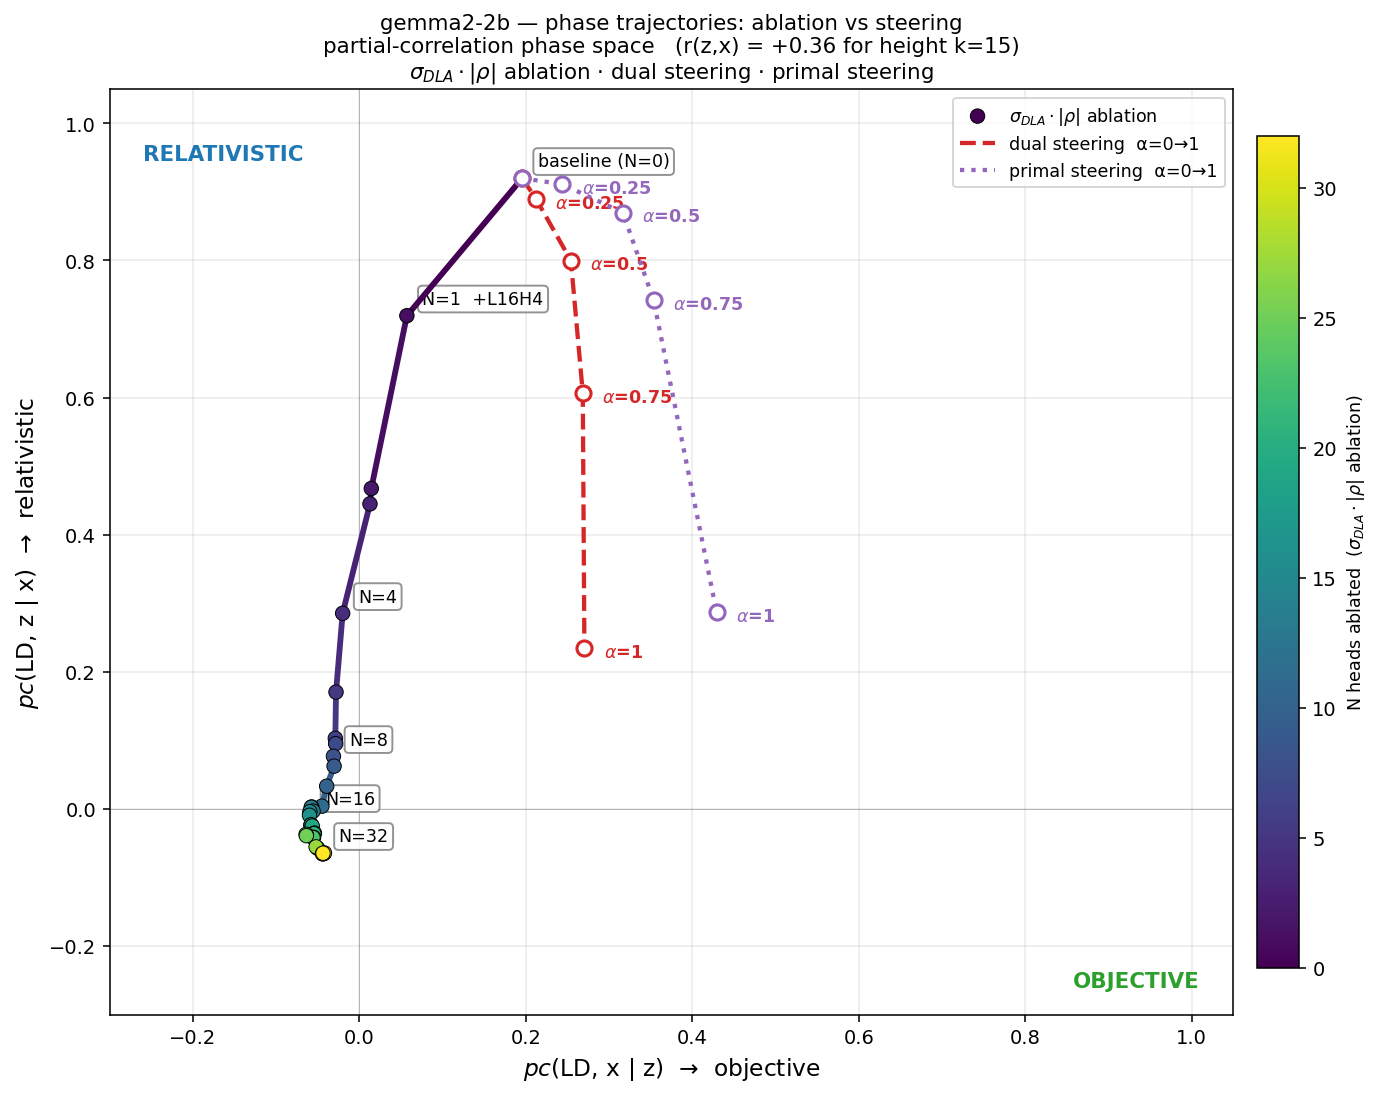
\includegraphics[width=\linewidth]{figures/p2v_phase_trajectory_partial_gemma2-2b.png}
  \caption{\textbf{Steering and ablation trace different routes out of the relativistic region on Gemma 2 2B.}
  The relative/objective phase plane of \cref{fig:relative-objective-phase}: We see clearly the different trajectories our intervention methods have, all removing relativistic behavior with various levels of maintaining objectivity. Dual steering is the cleanest way to univariately remove relativistic behavior.
  % Source artifact: relativity_ablation/figures/p2v_phase_trajectory_partial_gemma2-2b.png.
  }
  \label{fig:circuit-phase-trajectory}
\end{figure}

\subsection{Generalization Across Scale and Modalities}
\label{subsec:generalization}

All results, including the general decomposition into Z score relativity, the dense grid, as well as causal steering and attention based interventions, were replicated on a host of small models. These models included OLMO 7B, Pythia 2.8B, Llama 3.2 3B, Qwen 2.5 3B and Qwen 3 14B. Results were generally similar as reported in this paper on the Gemma 2 family models. 

The broader generalization question to larger models with more parameters remains largely open. Largest model we tested was 14B active parameters.


\section{Related Work and Positioning}
\label{sec:related-work}

\subsection{Gradable Adjectives and Pragmatic Thresholds}
\label{subsec:related-gradability}

Prior to the age of LLMs, a general pragmatic understanding of relativistic adjectives in natural language was studied. \citep{lassiter2017adjectival} provides a Bayesian framework for interpreting such types of adjectives. Recent LLM work and the discovery of in-context learning further test the inferential capabilities of Bayesian language models \citep{lipkin2023pragmatic}. Our work, built on these foundations, extensively focuses on interpreting how the comparisons and relativity are geometrically represented in the model's internals.

\subsection{Numerical Representations and In-Context Statistics}
\label{subsec:related-numbers}

Numeracy work shows that hidden states can encode numerical magnitude, but it also warns that notation, tokenization, base-10 digit structure, and verbalization failures can strongly shape what is measured \citep{wallace2019numbers,zhu2024value,levy2025base10,yuchi2026numbers}.
Measurement and numerical-attribute studies further show that language models mix numbers with world knowledge and contextual cues \citep{park2022measurements,takagi2025confounding}.
Our dense-grid design separates these factors by holding the adjective-pair task fixed while independently varying raw value and normalized standing.
The result is a direct test of whether the model uses the prompt numbers as isolated magnitudes or as samples from a local distribution.

This also connects to work on in-context learning as implicit statistical inference.
Prior theory and controlled mechanistic studies show that transformers can implement Bayesian-like, gradient-like, or estimator-like computations from examples \citep{xie2022implicitbayesian,muller2022bayesian,akyurek2023algorithm,vonoswald2023gradient,bai2023statisticians,he2025linearregression,chaudhry2026implicit}.
Our setting is less synthetic but more semantically natural: the context examples are ordinary scalar quantities, and the inferred statistic is the target's relative standing inside that local population.

\subsection{Linear Representations, Steering, and Manifold Geometry}
\label{subsec:related-mi}

Linear representations of concepts of natural language were a common starting point for mechanistic interpretability for a long time \citep{park2023lrh,park2025categorical}, linear methods such as probing and steering were actively used to connect the geometry of the linear representation to the behavior of the model.
However, more recent work shows that not all features are linearly defined; Certain features were discovered to require richer geometry such as cyclical, hierarchial, and low dimensional manifolds. \citep{engels2024notlinear,modell2025origins,sarfati2026beliefs,gurnee2026linebreaks}.

Our use of \primalz{} sits between these views. Concepts such as \emph{tall} vs \emph{short} could be interpreted as counterfactual;binary which is best represented linearly, whereas other interpretations might suggest it is based on a probability distribution which is represented in nonlinear manifolds \citep{sarfati2026beliefs}. Therefore whilst testing linear decodability and steerability and the downstream causal effects of $z$, we also deploy methods such as dual steering to exploit the nonlinearities of the geometric structures, rather than collapsing them into a single ``the model has a vector'' claim.

\section{Discussion and Limitations}
\label{sec:discussion-limitations}

\subsection{What This Paper Can Claim}
\label{subsec:can-claim}

The core result is that in-context scalar judgments are better described by a context-normalized variable than by raw magnitude alone.
The dense grid separates $x$ from $z$ by construction, and across eight adjective domains the model's high-minus-low logit differences track $z$ far more strongly than $x$.
The same variable is visible in activation geometry: cell-mean residual-stream states form ordered $z$ structure, and linear readouts recover $z$ early in the network.
These observations do not by themselves prove a mechanism, but they establish that the behavioral phenomenon and the internal geometry agree on the same normalized coordinate.
The shot-sweep phase-plane result adds an important behavioral refinement: with no comparison examples, the model behaves more like an objective magnitude reader, but even a small amount of context moves it toward a relative judgment regime.
This supports the interpretation that the model is not merely retrieving a fixed world prior, but dynamically changing the computation as the prompt supplies a comparison class.

The intervention results strengthen this interpretation.
Steering with \primalz{} changes adjective decisions in the predicted direction, and source-concept \primalz{} directions transfer more broadly than raw-$x$ directions.
The transfer is partial rather than complete: diagonal effects remain larger than off-diagonal effects, and lexical decomposition shows that same-concept steering receives high-gain support from adjective-specific and output-facing components.
We therefore interpret \primalz{} as an operational summary of a mixed representation: it contains a shared relative-standing component, but it is not a pure universal direction independent of lexical content.

The attention-intervention results provide a complementary causal view.
Direct zero-ablation of individual heads is mostly ineffective, consistent with redundancy once $z$ is widely linearly available.
Interchange resampling of DLA-ranked heads, by contrast, strongly reduces the relativity readout while preserving much of the ordinary next-token distribution on unrelated text.
The strongest heads transfer across several relativity concepts, suggesting a relativity-general computation rather than a height-specific trick.
Together with the steering results, this gives two different intervention paths into the same phenomenon: residual-stream directions can move the judgment along the relative coordinate, while attention resampling can selectively corrupt the route that carries context-relative information.

\subsection{What This Paper Cannot Claim Yet}
\label{subsec:cannot-claim}

The generalization evidence should also be read conservatively.
The same qualitative decomposition into raw magnitude, relative standing, steering, and attention-based intervention appears across several small model families, including OLMo, Pythia, Llama, Qwen, and Gemma variants.
This argues against the phenomenon being an idiosyncrasy of one Gemma checkpoint.
However, the largest tested model has 14B active parameters, and the present experiments do not yet establish scaling behavior, instruction-tuned robustness, multimodal generalization, or behavior under substantially more diverse semantic domains.

The attention intervention is not yet a complete circuit-level explanation.
It identifies important routing sites and failure modes, but it does not decompose the full algorithm by which the model estimates the comparison statistic from context.
In particular, we do not yet know whether the model explicitly represents $\mu$ and $\sigma$, computes a normalized statistic through a small set of reusable subroutines, or approximates the same behavior through a more distributed comparison process.

Several limitations remain.
First, the main behavioral readout is a high-minus-low logit difference over hand-chosen adjective tokens; future versions should test broader paraphrase sets and top-logit behavior.
Second, the domains are mostly scalar human-interpretable quantities, so stronger controls should include more distant physical, economic, and objective classification tasks.
Third, PCA, probes, steering, and ablations answer different questions; the paper deliberately separates them rather than treating any one method as definitive.
The current evidence supports a context-relative scalar representation that is behaviorally dominant, internally accessible, causally relevant, and partly shared across concepts, but it does not yet prove a single clean mechanism or a fully non-lexical code.

\section{Conclusion}
\label{sec:conclusion}

We use gradable adjectives as a controlled setting for studying how language models represent relational quantities in context.
By independently varying raw target value and normalized standing, we show that context examples induce a $z$-like coordinate that appears in behavior, activation geometry, steering, and attention interventions.
The central lesson is claim hygiene: relative standing is a real and causally relevant internal variable, but it is implemented through a mixed mechanism with lexical, residual, and attention-mediated components.

\section*{Impact Statement}

This paper presents work whose goal is to advance mechanistic understanding of machine learning systems.
It studies synthetic prompt tasks and does not introduce a deployed model, dataset of personal information, or decision procedure.
The main expected impact is methodological: the experiments provide a controlled way to distinguish raw numerical magnitude, context-normalized standing, linear decodability, causal steering, and attention-based intervention effects.
Clearer distinctions between these evidence types may help future interpretability work avoid overclaiming from probes, PCA visualizations, or single intervention methods.

The topic has potential relevance to fairness, calibration, and context use because many real decisions involve context-sensitive scalar comparisons.
For example, a system may need to distinguish an absolute value from a value that is high or low relative to a local distribution.
However, our experiments are limited to synthetic prompts over simplified scalar domains and should not be treated as evidence that current language models make reliable or fair context-sensitive judgments in deployed settings.
Any application to high-stakes domains would require separate validation, domain-specific measurements, and safeguards against harmful comparison classes.

There are also modest dual-use considerations.
The steering and ablation methods used here are intended as analysis tools, but similar techniques could be used to manipulate model behavior.
We mitigate this risk by studying small, non-deployed models and by framing interventions as diagnostic evidence rather than as a recipe for controlling deployed systems.

\bibliography{references}
\bibliographystyle{icml2026}

\appendix

\section{Definitions and Metrics}
\label{app:definitions}

\paragraph{Logit difference.}
For each adjective pair, the behavioral readout is
\[
\mathrm{LD}=\mathrm{logit}(\text{high adjective})-\mathrm{logit}(\text{low adjective}).
\]
Positive LD means the model leans toward the high adjective.

\paragraph{Cell means.}
Many analyses average activations or logits over context seeds inside each $(x,z)$ cell:
\[
\bar h_{x,z,L}=\mathbb{E}_{\mathrm{seed}}[h_{x,z,\mathrm{seed},L}].
\]
This reduces context-sampling noise and gives $400$ cell-mean points per pair in the dense grid.

\paragraph{Squared-correlation $R^2$.}
Unless explicitly marked as a cross-validated probe score, reported $R^2$ values are squared correlations:
\[
R^2(a,b)=\mathrm{corr}(a,b)^2.
\]

\paragraph{Partial-correlation phase axes.}
The relative/objective phase plots use partial correlations:
\[
r_{\mathrm{rel}}=\mathrm{corr}(\mathrm{LD},z\mid x),\qquad
r_{\mathrm{obj}}=\mathrm{corr}(\mathrm{LD},x\mid z).
\]
Operationally, $\mathrm{corr}(a,b\mid c)$ is computed by regressing $a$ and $b$ on $c$, then correlating the two residuals.
This asks whether LD still tracks $z$ after accounting for raw value, or still tracks raw value after accounting for $z$.

\paragraph{PCA $R^2$.}
PCA is fit to activation vectors $h_i\in\mathbb{R}^d$.
For a principal direction $v_{\mathrm{PC1}}$, each example receives a scalar score
\[
s_i=(h_i-\bar h)\cdot v_{\mathrm{PC1}}.
\]
Then $R^2(\mathrm{PC1},z)=\mathrm{corr}(s,z)^2$.
This is not PCA explained variance; it asks whether position along a PC orders examples by $z$.

\paragraph{SAE feature $R^2$.}
For SAE feature activation $a_{i,f}$:
\[
R^2(f,z)=\mathrm{corr}(a_f,z)^2,\quad
R^2(f,x)=\mathrm{corr}(a_f,x)^2.
\]
Numeric-token controls analogously correlate the feature activation with token-magnitude proxies.

\paragraph{Probe $R^2$.}
Probe results use a supervised linear model, typically ridge regression:
\[
\hat y = h w + b.
\]
When marked as cross-validated $R^2$, the score is held-out prediction quality, not in-sample correlation.

\paragraph{Mean-difference directions.}
For a pair and layer,
\[
d^{\mathrm{primal}}_{z,p,L}
= \mathbb{E}[h_L\mid p,z>1]-\mathbb{E}[h_L\mid p,z<-1].
\]
Analogously, \primalx{} compares high-$x$ and low-$x$ prompts and is used as a raw-value control.
This high-margin definition is the one used for the current dense-grid transfer and steering analyses.
Some older exploratory manifold scripts used a lower-margin sign split, $z>0$ minus $z<0$; those results should not be mixed with the current \primalz{} definition without restating the threshold.

\paragraph{Steering slopes.}
For unit direction $\hat d$, layer $L$, and intervention scale $\alpha$, steering adds or subtracts the direction:
\[
h'_L=h_L\pm \alpha\hat d.
\]
The reported slope is
\[
\frac{\mathbb{E}[\mathrm{LD}(h+\alpha\hat d)-\mathrm{LD}(h-\alpha\hat d)]}{2\alpha}.
\]
This is an intervention effect on logit difference per unit $\alpha$, not LD divided by a $z$ score.

\paragraph{Shared direction and cross-pair transfer.}
Each adjective pair has its own \primalz{} vector.
The shared direction is a sign-aligned mean of per-pair directions, used as a consensus above-vs-below-local-norm direction.
For source pair $s$ and target pair $t$, cross-pair transfer steers target prompts with the source pair's direction and reads the target pair's LD.

\section{Lexical Decomposition}
\label{app:lexical-decomposition}

For each pair, lexical directions are built from token-position captures such as adjective-token states, adjective-in-sentence states, sentence-final states, synonym-token contrasts, and domain-token contrasts.
Token-position captures use tokenizer offsets to average hidden states over the tokens overlapping the relevant word or phrase.
These directions form an orthonormal lexical basis:
\[
Q_L=\operatorname{orth}([d_1,\dots,d_k]).
\]
Normalize the context direction:
\[
p_z=\operatorname{unit}(\primalz).
\]
Project into the lexical subspace and take the residual:
\[
p_{z,\mathrm{lex}}=Q_LQ_L^\top p_z,\qquad
p_{z,\mathrm{resid}}=p_z-p_{z,\mathrm{lex}}.
\]
By construction, $p_{z,\mathrm{lex}}^\top p_{z,\mathrm{resid}}\approx 0$.
The lexical energy fraction is $\|p_{z,\mathrm{lex}}\|^2$ because $p_z$ is unit norm.

Steering uses normalized versions of the projection and residual.
Therefore a small lexical projection can steer more strongly than full \primalz{} if it points in a high-gain output-facing direction.
In the current 9B layer-33 follow-up, full \primalz{} has diagonal/off-diagonal means $+0.067/+0.026$, lexical projection has $+0.087/+0.011$, lexical residual has $+0.044/+0.024$, and a random null is approximately zero.
This supports a mixed mechanism: the residual carries broad cross-domain transfer, but target lexical-subspace leakage prevents a clean non-lexical claim.

\section{Dual Steering}
\label{app:dual-steering}

Dual steering is a per-prompt residual-stream intervention derived from the empirical activation manifold, contrasted with \emph{primal steering}, which adds a single fixed direction scaled by a scalar $\alpha$.

\paragraph{Motivation.}
Primal steering applies $h\leftarrow h\pm\alpha\,\hat d$ for a fixed unit direction $\hat d$ (typically \primalz). This is appropriate when the target attribute is encoded along a straight direction, but it is mismatched to a curved manifold or to a population whose $z$-direction varies with raw value $x$. Dual steering replaces the single direction by a \emph{per-prompt displacement} $\Delta_i$ read off the model's own cell-mean structure.

\paragraph{Cell-mean lookup.}
For each pair and layer $L$, split the dense $(x,z)$ grid by context seed into a training fold (e.g.\ \texttt{cell\_seed}\,$\in\{0,1,2,3,4\}$) and a test fold ($\{5,6,7,8,9\}$).
On the training fold, build a cell-mean lookup
\[
M_L(x,z)=\mathbb{E}_{\mathrm{seed}\in\text{train}}\bigl[h_L\mid x,z\bigr],
\]
indexed by the rounded $(x,z)$ cell key.
Cells with no training prompts are absent from the lookup; in our v11 grid the train and test folds share the same $(x,z)$ skeleton so this never triggers.

\paragraph{Displacement.}
For a test prompt with cell $(x_i,z_i)$ and a target $z_{\text{target}}$ (default $z_{\text{target}}=0$, corresponding to the \emph{objective} cell on the same-$x$ slice), compute
\[
\Delta_i \;=\; M_L\!\bigl(x_i,\;z^\star_i\bigr)\;-\;M_L\!\bigl(x_i,\;z_i\bigr), \qquad
\]
\[
z^\star_i \;=\;\operatorname*{arg\,min}_{z\in\mathcal{Z}(x_i)}\bigl|z-z_{\text{target}}\bigr|,
\]
where $\mathcal{Z}(x_i)$ is the set of $z$ values populated on the same-$x_i$ slice of $M_L$.
Source cell defaults to $M_L(x_i,z_i)$; if that cell is missing, the nearest-$z$ same-$x$ cell is used as a fallback. The displacement therefore moves each prompt along the empirical manifold toward its same-$x$ objective neighbour, preserving raw value $x$ while collapsing $z$.

\paragraph{Intervention.}
At the chosen layer $L$, hook the residual stream and add the per-prompt displacement, broadcast across all token positions:
\[
h_{L,i,t} \;\leftarrow\; h_{L,i,t}\;+\;\alpha\,\Delta_i,
\qquad t\in\{1,\dots,T\}.
\]
Setting $\alpha=1$ realises the full manifold shift to $z_{\text{target}}$; intermediate $\alpha$ traces out the trajectory between the prompt's natural cell and the target cell. The shift is identical on every token; what varies across prompts is the direction \emph{and} magnitude of $\Delta_i$, both derived from $M_L$.

\paragraph{Comparators.}
Each dual-steering evaluation is reported alongside three controls held to the same test fold and the same hooked layer:
\begin{enumerate}
\item \textbf{Baseline:} no hook.
\item \textbf{Per-pair project-out:}
$h\leftarrow h-(h\cdot\hat d_p)\,\hat d_p$ with
$\hat d_p=\operatorname{unit}(\primalz)$ from the training fold. Removes a
rank-one $z$-direction with no manifold information.
\item \textbf{Random matched:} $h\leftarrow h+\alpha\,r_i$ where $r_i$ is a uniform unit vector in $d$ dimensions rescaled to match $\|\Delta_i\|$.
This holds the per-prompt magnitude profile fixed and tests whether the \emph{direction} of $\Delta_i$ matters.
\end{enumerate}

\paragraph{Readouts.}
On the test fold, report partial correlations $r(\mathrm{LD},z\mid x)$ and $r(\mathrm{LD},x\mid z)$ as defined in Appendix~\ref{app:definitions}, together with the unconditional correlations and $\langle\mathrm{LD}\rangle$. A successful dual-steering intervention drives $r(\mathrm{LD},z\mid x)$ toward zero without inducing a compensating raw-value reading $r(\mathrm{LD},x\mid z)$, and without large shifts in $\langle\mathrm{LD}\rangle$ (the population mean is preserved by the same-$x$ construction).

\paragraph{$\alpha$-sweep.}
The trajectory plots in the main text vary $\alpha\in\{0.0, 0.25, 0.5, 0.75, 1.0\}$ with $\Delta_i$ fixed. At $\alpha=0$ this recovers the baseline; at $\alpha=1$ it realises the full manifold shift. The sweep is anchored to the baseline $(r_x,r_z)$ point so that primal- and dual-steering trajectories share a common origin in the phase plane.

\paragraph{Naming.}
Earlier internal versions of this analysis (Phase 1d/1e/2E in our logs) called the same intervention \emph{manifold shift} or \emph{on-manifold tangent ablation}; we use \emph{dual steering} throughout the paper to emphasise its role as the dual of primal direction-based steering. ``Primal'' (single direction, scalar $\alpha$) and ``dual'' (per-prompt manifold displacement) are paired interventions on the same hooked layer with the same readouts; differences in efficacy are interpretable as evidence about whether the encoding is a single linear direction or a curved manifold.


\end{document}
